One constraint in this project is to build two different classifiers to compare their efficiency. So we choose to build one classifier based on the style of writing (punctuation, number of words per sentence ...) and one based on the content of the article (adjectives, common words...).

Here is a graphical recap of how the project is structured.
\begin{figure}[h]
	\centering
		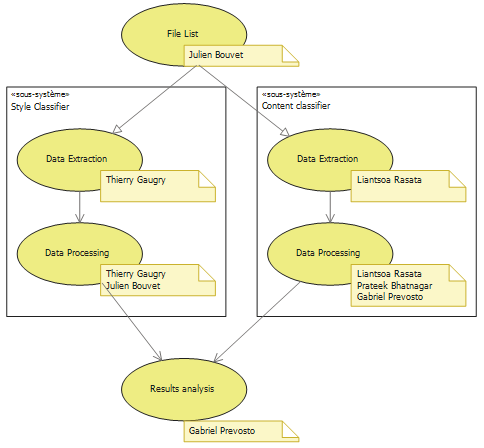
\includegraphics{Images/organization.png}
	\caption{Organization}
	\label{fig:organization}
\end{figure}

The first step is to build the list of the files, that the algorithms will need to retrieve some good information for the classifiers.\\
Then, from the files given by the previous step, we'll extract data for the first classifier (\ref{lab:data1}) and for the second (\ref{lab:data2}). This step creates a new, understanding representation of the articles, based on its classifier features.\\
After that, the style based classifier (\ref{lab:clas1}) or the content based classifier\ref{lab:clas2} will use all this data to decide who is the author of a given text.\\
To finish this, we added a results analysis (\ref{lab:ana}) step, to understand what is actually working or not, and compare the two classifiers.
